\textbf{02/04/2025}
\section{Clase 21}

\subsection{Método egipcio para el cálculo de un número (falsa posición)}
Problema 26 del Papiro matemático Rhind (1650 a.C.).Una cantidad y su cuarta parte se convierten en 15. 

En esencia es resolver una ecuación lineal. Los escribas egipcios lo resolvían mediante la «posición falsa»

\par
\begin{minipage}[t]{0.48\textwidth}
    Lo primero que se hacía era suponer un número que pudiese cumplir el problema, en este caso, sea 4 entonces $4 + \frac{4}{4} = 5$. Aunque este número no resuelve la cantidad, notemos que $5\times 3 = 15$ Así $4 \times 3+ \frac{4\times 3}{4} = 5\times3 = 15$
\end{minipage}
\begin{minipage}[t]{0.48\textwidth}
    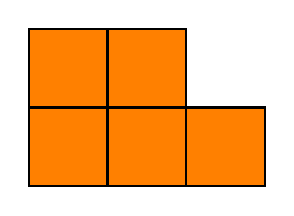
\begin{tikzpicture}
    \draw[fill = orange,thick] (0,0) -- (1,0) -- (1,1) -- (0,1) --cycle;
    \draw[fill = orange,thick] (0,1) -- (1,1) -- (1,2) -- (0,2) --cycle;
    \draw[fill = orange,thick] (1,0) -- (2,0) -- (2,1) -- (1,1) --cycle;
    \draw[fill = orange,thick] (1,1) -- (2,1) -- (2,2) -- (1,2) --cycle;
    \draw[fill = orange,thick] (2,0) -- (3,0) -- (3,1) -- (2,1) --cycle;
\end{tikzpicture}
\end{minipage}
\par

\subsection{Sistema de ecuaciones por el método chino}
El séptimo problema del capítulo 8 del Jiuzhang suanshu (c. 100 a.C.) dice lo siguiente: Tenemos cinco vacas y dos ovejas que cuestan 10 liang de plata. Dos vacas y cinco ovejas cuestan 8 liang de plata. ¿Cuánto cuestan una vaca y una oveja, respectivamente?

\textbf{Solución.} La solución era crear algo como lo siguiente\\
\begin{tabular}{c|cc|}
    Vacas  & 5 & 2 \\
    Ovejas  & 2 & 5 \\
    Costo  & 10 & 8\\
\end{tabular}
\\Si se busca hallar el costo de las ovejas, entonces se tiene que igualar la cantidad de vacas en ambas columnas, es decir la primera columna se multiplica por 2 y la segunda por 5\\
\begin{tabular}{c|cc|}
    Vacas  & 10 & 10 \\
    Ovejas  & 4 & 25 \\
    Costo  & 20 & 40\\
\end{tabular}
\\Se halla la diferencia de la cantidad de ovejas y la diferencia del costo y se igualan
\[
    21O_{v} = 20 \rightarrow O_{v} = \frac{20}{21}
\]
\\Análogamente para el costo de las ovejas\\
\begin{tabular}{c|cc|}
    Vacas  & 25 & 4 \\
    Ovejas  & 10 & 10 \\
    Costo  & 50 & 16\\
\end{tabular}
\[
    21V = 34 \rightarrow V = \frac{34}{21}
\]

Y con el método algebraico actual se llega al mismo resultado, aunque de forma más lenta.\\\\
Sea $x$ el costo de una vaca, y $y$ el costo de una oveja. Entonces:

\begin{align*}
5x + 2y &= 10 \quad \text{(ecuación 1)} \\
2x + 5y &= 8  \quad \text{(ecuación 2)}
\end{align*}

Multiplicamos la ecuación (1) por 5 y la ecuación (2) por 2 para igualar los coeficientes de $y$:

\begin{align*}
5(5x + 2y) &= 5(10) \Rightarrow 25x + 10y = 50 \quad \text{(ecuación 3)} \\
2(2x + 5y) &= 2(8) \Rightarrow 4x + 10y = 16 \quad \text{(ecuación 4)}
\end{align*}
Restamos las ecuaciones (3) y (4)

\begin{align*}
(25x + 10y) - (4x + 10y) &= 50 - 16 \\
21x &= 34 \\
x &= \frac{34}{21}
\end{align*}
Sustituimos $x$ en un la ecuación (1)

\begin{align*}
5x + 2y &= 10 \\
5\left(\frac{34}{21}\right) + 2y &= 10 \\
\frac{170}{21} + 2y &= 10 \\
2y &= 10 - \frac{170}{21} = \frac{210 - 170}{21} = \frac{40}{21} \\
y &= \frac{20}{21}
\end{align*}
El precio de una vaca es $\frac{34}{21}$
El precio de una oveja es $\frac{20}{21}$

\subsection{Problema algebraico de al-Khwarizmi}
Se trata de un problema sacado del Álgebra de al-Khwarizmi (c.830): Un cuadrado y diez veces su raíz equivalen a 39 dírhams. ¿Cuál es el valor de la raíz?
\par
\begin{minipage}[t]{0.48\textwidth}
Para resolverlo usaban figuras geométricas, en este caso se consideran dos rectángulos de igual tamaño, donde un lado mide 5 y el otro lado se desconoce su longitud.
Los rectángulos se acomodan perpendicularmente y se extienden sus lados de tal manera que se forme un cuadrado. Sabemos que por la construcción hecha, el área azul vale 25; y por hipótesis, $39+25=64$. El lado del cuadrado más grande debe valer 8, de donde se desprende que el lado del rectángulo debe valer 3.
\end{minipage}
\begin{minipage}[t]{0.48\textwidth}
    \begin{center}
        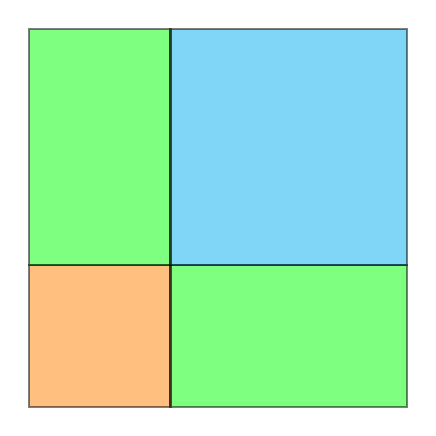
\begin{tikzpicture}[baseline=(current bounding box.north),scale=0.6]
    % cuadradito
    \draw[fill = orange, thick, opacity=0.5] (0,0) -- (3,0) -- (3,3) -- (0,3) --cycle;

    % ractangulos raices
    \draw[fill = green, thick, opacity=0.5] (3,0) -- (8,0) -- (8,3) -- (3,3) --cycle;
    \draw[fill = green, thick, opacity=0.5] (0,3) -- (0,8) -- (3,8) -- (3,3) --cycle;

    % Cuadrado 25

    \draw[fill = cyan, thick, opacity=0.5] (3,3) -- (8,3) -- (8,8) -- (3,8) --cycle;

\end{tikzpicture}
    \end{center}
\end{minipage}
\par

\subsection{Problema 2 del libro Propositiones ad Acuendos Juvenes}

Problema 2 del libro Propositiones ad Acuendos Juvenes, silo IX cuya autoría se le atribuye a
Alcuino de York.\\ Un hombre que iba por el camino vio a otros hombres que iban hacía él y les dijo: Si fueseis otros tantos como sois y se añadiese la mitad de la mitad de estos y depués se añadiese la mitad de este número, entonces conmigo seríamos cien. ¿Cuántos hombres vio el caminante?

La solución del problema consta en construir una representación gráfica, donde el área sombreada en naranja en la figura de abajo representa a la cantidad de hombres que se vió y las otras áreas representan lo que el problema plantea. En total el area sombreada de color azul de la figura de la derecha representa a 99 personas y el área total se puede divir en 11 partes iguales, por lo que el area de cada cuadrado peequeño es 9. Así, se sabe que el hombre vio a 36 personas.

\par
\begin{minipage}[t]{0.48\textwidth}
    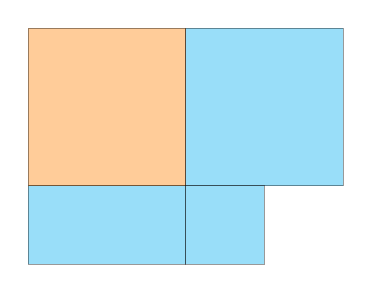
\begin{tikzpicture}
    \coordinate (A) at (0,0);
    \coordinate (B) at (2,0);
    \coordinate (C) at (2,1);
    \coordinate (D) at (0,1);
    \coordinate (E) at (0,3);
    \coordinate (F) at (2,3);
    \coordinate (G) at (4,3);
    \coordinate (H) at (4,1);
    \coordinate (I) at (3,0);
    \coordinate (J) at (3,1);

    \draw[fill = cyan, thin, opacity=0.4] (A) -- (B) -- (C) -- (D) --cycle;
    \draw[fill = orange, thin, opacity=0.4] (D) -- (C) -- (F) -- (E) --cycle;
    \draw[fill = cyan, thin, opacity=0.4] (C) -- (H) -- (G) -- (F) --cycle;
    \draw[fill = cyan, thin, opacity=0.4] (B) -- (I) -- (J) -- (C) --cycle;
\end{tikzpicture}
\end{minipage}
\begin{minipage}[t]{0.48\textwidth}
    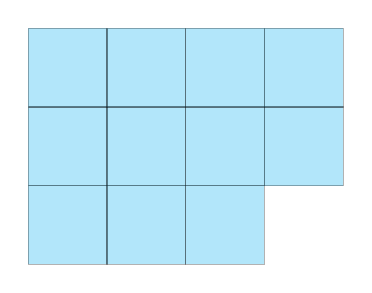
\begin{tikzpicture}
    \coordinate (A) at (0,0);
    \coordinate (B) at (2,0);
    \coordinate (C) at (2,1);
    \coordinate (D) at (0,1);
    \coordinate (E) at (0,3);
    \coordinate (F) at (2,3);
    \coordinate (G) at (4,3);
    \coordinate (H) at (4,1);
    \coordinate (I) at (3,0);
    \coordinate (J) at (3,1);
    \coordinate (K) at (1,0);
    \coordinate (L) at (1,1);
    \coordinate (M) at (0,2);
    \coordinate (N) at (1,2);
    \coordinate (O) at (2,2);
    \coordinate (P) at (3,2);
    \coordinate (Q) at (4,2);
    \coordinate (R) at (1,3);
    \coordinate (S) at (3,3);

    \draw[fill=cyan,thin,opacity=0.3] (A) -- (K) -- (L) -- (D) --cycle;
    \draw[fill=cyan,thin,opacity=0.3] (K) -- (B) -- (C) -- (L) --cycle;
    \draw[fill=cyan,thin,opacity=0.3] (B) -- (I) -- (J) -- (C) --cycle;
    \draw[fill=cyan,thin,opacity=0.3] (D) -- (L) -- (N) -- (M) --cycle;
    \draw[fill=cyan,thin,opacity=0.3] (L) -- (C) -- (O) -- (N) --cycle;
    \draw[fill=cyan,thin,opacity=0.3] (C) -- (J) -- (P) -- (O) --cycle;
    \draw[fill=cyan,thin,opacity=0.3] (J) -- (H) -- (Q) -- (P) --cycle;
    \draw[fill=cyan,thin,opacity=0.3] (M) -- (N) -- (R) -- (E) --cycle;
    \draw[fill=cyan,thin,opacity=0.3] (N) -- (O) -- (F) -- (R) --cycle;
    \draw[fill=cyan,thin,opacity=0.3] (O) -- (P) -- (S) -- (F) --cycle;
    \draw[fill=cyan,thin,opacity=0.3] (P) -- (Q) -- (G) -- (S) --cycle;
\end{tikzpicture}
\end{minipage}
\par

De forma algebraica es como siguiente

\begin{gather*}
    x+x+\frac{x}{2}+\frac{x}{4}+1=100 \\
    2x+\frac{3x}{4} = 99 \\
    \frac{11x}{4} = 99 \\
    x = \frac{4\cdot9\cdot11}{11} \\
    x = 36
\end{gather*}